\documentclass[11pt]{article}
\usepackage[margin=1in]{geometry}
\usepackage{amsmath,amssymb,amsthm,mathtools}
\usepackage{tikz}
\usepackage{booktabs}
\usepackage[T1]{fontenc}
\usepackage{lmodern}
\usepackage[colorlinks=true,linkcolor=blue!50!black]{hyperref}

\definecolor{cpar}{HTML}{0072B2}
\definecolor{crecv}{HTML}{D55E00}
\definecolor{csend}{HTML}{009E73}
\definecolor{cquote}{HTML}{CC79A7}
\definecolor{cdrop}{HTML}{56B4E9}
\definecolor{c0}{HTML}{000000}
\definecolor{cy}{HTML}{E69F00}
\tikzset{hub/.style={circle,inner sep=2.1pt,draw=white,line width=0.4pt},
         lab/.style={anchor=south west,inner sep=2.5pt}}

\newtheorem{theorem}{Theorem}
\newtheorem{lemma}[theorem]{Lemma}
\newtheorem{proposition}[theorem]{Proposition}
\theoremstyle{definition}
\newtheorem{definition}[theorem]{Definition}
\newtheorem{finding}{Finding}
\theoremstyle{remark}
\newtheorem{remark}[theorem]{Remark}

\newcommand{\R}{\mathbb{R}}
\newcommand{\ar}{\mathsf{ar}}
\newcommand{\sh}{\mathsf{s}}
\newcommand{\rad}{r}
\newcommand{\hgt}{\mathsf{h}}

\title{A Geometric Rendering of GSLT Syntax\\[2pt]\large Review, formal specification, and analysis}
\author{Prepared for L.\,G.\ Meredith}
\date{11 November 2026}

\begin{document}
\maketitle

\begin{abstract}
The proposed procedure assigns to each term of a graph-structured lambda theory a
figure made of line segments: one axis per constructor, arguments placed at the
vertices of a simplex, and a ``stem'' along the constructor's axis. This note
reviews the definition, fixes its underdetermined parts, and analyses the result.
The literal definition is \emph{faithful} on every term tested but is \emph{not an
embedding}: unary and binary constructors make segments overlap. A small change,
moving the hub from the barycentre of the simplex to the right-angled apex over it,
gives a construction that is provably an embedding and provably decodable. A
further variant makes one-hole contexts act as similarity maps, which is the
property needed if rewrites are to be rendered as local moves. Finally, moving
the constructor from a spatial axis to a colour brings the ambient dimension down
to the largest arity; for the rho calculus that is three, and
Section~\ref{sec:rho} works the example.
\end{abstract}

\section{Scope}

A GSLT presents a term language (a lambda theory: sorts, constructors, variables,
equations) with a graph of rewrites adjoined. The procedure under review concerns
the \emph{first-order, equation-free} part: closed terms built from constructors.
Sections~\ref{sec:spec}--\ref{sec:analysis} stay within that part;
Section~\ref{sec:beyond} says what happens to variables, binders, equations and
rewrites, and Section~\ref{sec:rho} renders a rho-calculus term in three
dimensions.

Fix a signature: a finite set $C$ of constructors with arities $\ar(c)\ge 0$.
Sorts are ignored, since a constructor determines its sorts; the rendering is
simply restricted to well-sorted terms. Write $\hgt(t)$ for the height of a term
($\hgt(z)=0$ for nullary $z$).

\section{Review of the definition as stated}\label{sec:review}

Reading the procedure literally raises five points that a specification must
settle. None of them is a matter of taste; each leaves the figure undefined or
changes it.

\begin{finding}[Simplex dimension]
$n$ arguments give $n$ vertices, which span an $(n-1)$-simplex, not an
$n$-simplex.
\end{finding}

\begin{finding}[Not enough axes]
With exactly one axis per constructor the ambient space is $\R^{|C|}$, and the
definition does not say in which directions the simplex for $c$ extends. A
regular $(n-1)$-simplex needs $n-1$ dimensions, and if those are borrowed from
other constructors' axes, the stems of those constructors run through it. The
canonical remedy is to give $c$ a block of $\max(1,\ar(c))$ axes
$e_{c,1},\dots,e_{c,n}$: the simplex is the standard one in that block, and ``the
direction of $c$'' is the block diagonal $u_c = n^{-1/2}\sum_i e_{c,i}$, which is
orthogonal to the simplex. Argument position $i$ is then recorded by the axis
$e_{c,i}$.
\end{finding}

\begin{finding}[Which barycentre]
``The barycentre of $\sh(t_i)$'' can mean the centre of mass of the figure or its
distinguished centre. Under the centre-of-mass reading the spokes end at points
that are generally not on the child figure, so the result is disconnected. The
specification below takes every shape to be \emph{pointed}: it carries a
\emph{hub}, and all references to the barycentre of a sub-shape mean its hub.
\end{finding}

\begin{finding}[Margins]
``Such that no $\sh(t_i)$ touches $\sh(t_j)$'' and ``just outside the smallest
sphere'' describe open conditions with no least solution. Two parameters are
needed: a sibling gap $\gamma>0$ and a stem overshoot $\delta>0$. Taking
$\delta=1$ makes the nullary rule an instance of the general one, since the
enclosing sphere of an empty assembly has radius $0$.
\end{finding}

\begin{finding}[Degenerate arities]
For $n=1$ the simplex is a point, so the hub of $c(t)$ coincides with the hub of
$t$. For $n=2$ the two spokes are opposite, so every nesting of a binary
constructor lies along one line. Both cases make segments overlap
(Section~\ref{sec:analysis}).
\end{finding}

\section{Formal specification}\label{sec:spec}

\begin{definition}[Pointed shape]
A \emph{pointed shape} in a Euclidean space $V$ is a pair $(S,\rad)$ where
$S\subset V$ is a finite union of closed segments containing the origin (the
\emph{hub}) and $\rad\ge\max_{x\in S}|x|$ is a bounding radius. For $v\in V$,
$v+S$ is the translate.
\end{definition}

\subsection{Realisation A: barycentric (the definition as stated)}

Let $V_A=\bigoplus_{c\in C}\R^{\max(1,\ar(c))}$ with orthonormal basis
$e_{c,i}$, and for $\ar(c)=n\ge1$ put
\[
u_c=\tfrac{1}{\sqrt n}\textstyle\sum_{i}e_{c,i},\qquad
w_{c,i}=\frac{e_{c,i}-\frac1n\sum_j e_{c,j}}{\sqrt{(n-1)/n}}\ \ (n\ge2),\qquad
\kappa_n=\sqrt{\tfrac{n-1}{2n}} .
\]
The $w_{c,i}$ are the unit directions from the centre of a regular
$(n-1)$-simplex to its vertices, and $\kappa_n$ is its circumradius per unit edge.
For nullary $z$, $u_z$ is the single axis of its block.

\begin{definition}[Realisation A]\label{def:A}
For $t=c(t_1,\dots,t_n)$ with $\sh_A(t_i)=(S_i,\rad_i)$ and
$\rad_{\max}=\max_i\rad_i$ (and $\rad_{\max}=0$, $\ell=0$ when $n=0$):
\begin{align*}
\ell &= 2\rad_{\max}+\gamma, &
\rho &= \kappa_n\ell+\rad_{\max}\ \ (\rho=0 \text{ if } n=0),\\
S &= [0,(\rho+\delta)u_c]\ \cup\ \bigcup_{i=1}^n\Bigl([0,\kappa_n\ell\,w_{c,i}]\cup(\kappa_n\ell\,w_{c,i}+S_i)\Bigr), &
\rad &= \rho+\delta .
\end{align*}
Then $\sh_A(t)=(S,\rad)$.
\end{definition}

Here $\ell$ is the edge of the simplex $b(t)$, the hub is its barycentre, the
segments $[0,\kappa_n\ell\,w_{c,i}]$ are the spokes and $[0,(\rho+\delta)u_c]$ is
the stem. The radius $\rho$ is a hub-centred bound on the assembly of children
rather than the exact smallest enclosing sphere; the bound has a closed recurrence
and still guarantees that the stem tip lies outside.

\subsection{Realisation B: corner (the repair)}

Let $V_B=\bigoplus_{c\in C}\R^{1+\ar(c)}$ with orthonormal basis
$e_{c,0},e_{c,1},\dots,e_{c,n}$. The axis $e_{c,0}$ is ``the dimension of $c$''.

\begin{definition}[Realisation B]\label{def:B}
For $t=c(t_1,\dots,t_n)$ with $\sh_B(t_i)=(S_i,\rad_i)$:
\begin{align*}
\lambda &= \sqrt2\,\rad_{\max}+\gamma, &
\rho &= \lambda+\rad_{\max}\ \ (\rho=0 \text{ if } n=0),\\
S &= [0,(\rho+\delta)e_{c,0}]\ \cup\ \bigcup_{i=1}^n\Bigl([0,\lambda e_{c,i}]\cup(\lambda e_{c,i}+S_i)\Bigr), &
\rad &= \rho+\delta .
\end{align*}
\end{definition}

The child hubs $\lambda e_{c,1},\dots,\lambda e_{c,n}$ are still the vertices of a
regular $(n-1)$-simplex, of edge $\sqrt2\lambda$. The only departure from the
stated procedure is that the hub sits at the apex of the right-angled pyramid over
that simplex instead of at its barycentre, and the stem leaves along its own axis.

\section{Analysis}\label{sec:analysis}

Let $T^+(t)$ be the syntax tree of $t$ with one extra pendant edge (the stem)
at every node. A realisation is an \emph{embedding} if distinct edges of $T^+(t)$
are sent to segments that meet only in a shared endpoint, and \emph{faithful} if
$t\mapsto S$ is injective.

\subsection{Realisation A is not an embedding}

\begin{proposition}\label{prop:Afail}
Realisation A fails to be an embedding for every signature containing a unary or
a binary constructor.
\end{proposition}
\begin{proof}
\emph{Unary.} $\kappa_1=0$, so in $u(u(z))$ both $u$-nodes have hub $0$ and their
stems $[0,2u_u]$ and $[0,3u_u]$ overlap.
\emph{Binary.} $w_{b,2}=-w_{b,1}$. In $b(b(z,z),z)$ the inner node has hub
$4w_{b,1}$ and places its second leaf at $4w_{b,1}-1.5\,w_{b,1}=2.5\,w_{b,1}$,
which is an interior point of the outer spoke $[0,4w_{b,1}]$
(Figure~\ref{fig:comb}, with $\gamma=\delta=1$).
\end{proof}

\begin{figure}[h]
\centering
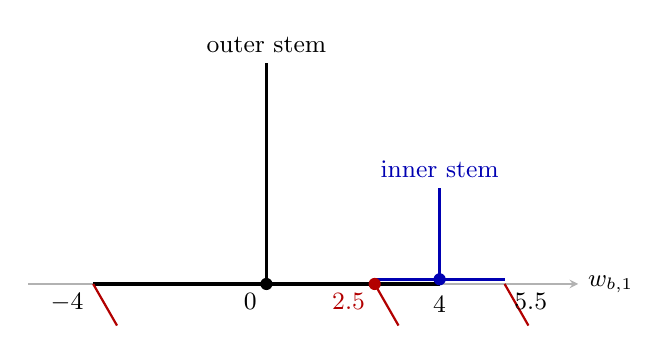
\begin{tikzpicture}[x=0.55cm,y=0.33cm,>=stealth]
  \draw[gray!60,->] (-5.5,0)--(7.2,0) node[right,black]{\small $w_{b,1}$};
  \draw[very thick] (-4,0)--(4,0);
  \draw[very thick,blue!70!black] (2.5,0.18)--(5.5,0.18);
  \draw[very thick] (0,0)--(0,8.5) node[above]{\small outer stem};
  \draw[very thick,blue!70!black] (4,0.18)--(4,3.68) node[above]{\small inner stem};
  \foreach \x in {-4,2.5,5.5} \draw[thick,red!70!black] (\x,0)--++(0.55,-1.6);
  \fill (0,0) circle(2.2pt) node[below left]{\small $0$};
  \fill[blue!70!black] (4,0.18) circle(2.2pt);
  \fill[red!70!black] (2.5,0) circle(2.2pt) node[below left]{\small $2.5$};
  \node[below] at (4,-0.1) {\small $4$};
  \node[below right] at (5.5,0) {\small $5.5$};
  \node[below left] at (-4,0) {\small $-4$};
\end{tikzpicture}
\caption{Realisation A of $b(b(z,z),z)$. The inner node's spokes (blue, drawn
slightly raised) lie on the same line as the outer spokes (black); the leaf at
$2.5$ sits in the interior of the outer spoke. Red: unit stems of the leaves
along $u_z$.}\label{fig:comb}
\end{figure}

A computational check over a signature with one constructor of each arity
$0,1,2,3$ (all $85$ terms of height $\le2$ and $400$ random terms of height $3$
and $4$) agrees: $252$ of the $485$ figures have segments in improper contact.
In separate samples, $38$ of $40$ binary-only terms have contact, and none of
$101$ ternary-only terms do. So the failure is confined to arities $1$ and $2$ in
everything tested; for $n\ge3$ the incoming spoke points at the centre of the
opposite face of the child simplex and passes between the grandchildren.

\begin{remark}[A is still faithful where tested]
The same $485$ figures are pairwise distinct as point sets. Lengths rescue
injectivity: each level of nesting strictly lengthens the stem, so $u(u(z))$ is
told from $u(z)$ by a stem of length $3$ rather than $2$. That is a metric
encoding rather than a geometric one, and it is not proved here in general.
\end{remark}

\subsection{Realisation B is an embedding and is decodable}

\begin{lemma}\label{lem:orthant}
For every $t$, $\sh_B(t)=(S,\rad)$ satisfies $S\subset\R_{\ge0}^{\dim V_B}$ and
$|x|\le\rad$ for all $x\in S$.
\end{lemma}
\begin{proof}
Induction. Every displacement is a non-negative multiple of a basis vector, and a
point $\lambda e_{c,i}+x$ with $x\in S_i$ has norm at most
$\lambda+\rad_i\le\rho<\rad$.
\end{proof}

\begin{theorem}[Embedding]\label{thm:emb}
Realisation B is an embedding of $T^+(t)$ for every term $t$.
\end{theorem}
\begin{proof}
Induction on $t$; the nullary case is one segment. Let $t=c(t_1,\dots,t_n)$ and
$B_i$ the closed ball of radius $\rad_i$ about $\lambda e_{c,i}$, which contains
$\lambda e_{c,i}+S_i$ by Lemma~\ref{lem:orthant}.
(i)~\emph{Siblings.} For $i\ne j$ the centres are $\sqrt2\lambda
=2\rad_{\max}+\sqrt2\gamma>\rad_i+\rad_j$ apart, so $B_i\cap B_j=\emptyset$.
(ii)~\emph{Spoke or stem against another child.} A point $s\,e_{c,k}$ with
$k\ne j$ lies at distance $\sqrt{s^2+\lambda^2}\ge\lambda>\rad_j$ from
$\lambda e_{c,j}$, so spoke $i$ and the stem miss $B_j$ for $j\ne i$.
(iii)~\emph{Spoke against its own child.} If $s\,e_{c,i}=\lambda e_{c,i}+x$ with
$x\in S_i$ and $s<\lambda$, then $x=(s-\lambda)e_{c,i}$ has a negative
coordinate, contradicting Lemma~\ref{lem:orthant}. So spoke $i$ meets its child
only at the child's hub.
(iv)~The stem and spokes are mutually orthogonal and meet only at $0$.
\end{proof}

\begin{theorem}[Faithfulness and decoding]\label{thm:faith}
$t\mapsto\sh_B(t)$ is injective, and $t$ is recovered from the point set $S$ by a
recursive procedure.
\end{theorem}
\begin{proof}
By Theorem~\ref{thm:emb}, exactly one segment in a direction of the form
$e_{d,0}$ leaves the hub; it names the head constructor $c$. For each
$i\le\ar(c)$, follow the ray from the hub along $e_{c,i}$: the hub of the $i$-th
argument is the first point at which a segment in some direction $e_{d,0}$ is
attached. Such a point exists because every hub carries a stem, and no stem
attaches earlier because edges meet only at endpoints. Recurse.
\end{proof}

\subsection{Size}

Both realisations fix leaves at unit size and grow outwards, so the radius
depends on height.

\begin{proposition}\label{prop:size}
With $\gamma=\delta=1$: in Realisation B,
$\rad(t)=(1+\sqrt2)^{\hgt(t)+1}-\sqrt2$ for every term. In Realisation A,
$\rad(t)=(1+2\kappa_n)\rad_{\max}+\kappa_n\gamma+\delta$ at a node of arity $n$;
for a purely binary term $\rad(t)=\tfrac52\,2^{\hgt(t)}-\tfrac32$.
\end{proposition}
\begin{proof}
B: $\rad=(1+\sqrt2)\rad_{\max}+2$ with $\rad=1$ at leaves, and $\rad_{\max}$
is attained at a child of maximal height. A: substitute in
Definition~\ref{def:A}.
\end{proof}

\begin{center}
\begin{tabular}{lccc}
\toprule
 & ambient dimension & growth per level & embedding \\
\midrule
A (barycentric) & $\sum_c\max(1,\ar(c))$ & $1+2\kappa_n\in[2,\,1+\sqrt2)$, \ $1$ if $n=1$ & no ($n\le2$) \\
B (corner) & $\sum_c(1+\ar(c))$ & $1+\sqrt2\approx2.41$ & yes \\
D (chromatic, \S\ref{sec:rho}) & $\max_c\ar(c)$ & $1+\sqrt2$ & yes \\
\bottomrule
\end{tabular}
\end{center}

Three consequences follow.
\begin{itemize}
\item The radius is exponential in height. For balanced terms that is polynomial
in term size (linear for binary terms under A), but for a comb such as
$P_1\mid(P_2\mid(\cdots))$ it is exponential in size, because the regular simplex
is scaled by the \emph{largest} child even when the others are leaves.
\item The ratio of the largest to the smallest feature is about $2.4^{\hgt}$. A
height of roughly $40$ exhausts double precision.
\item For a rho-calculus-like signature ($0$, parallel, send, receive, quote,
dereference, with arities $0,2,2,3,1,1$) the ambient dimension is $10$ under A
and $15$ under B. Anything shown on a screen is a projection.
\end{itemize}

\begin{remark}[Projection]
A generic linear projection $V\to\R^3$ keeps disjoint segments disjoint, so an
embedded figure stays embedded in three dimensions and can still be decoded from
the images of the basis vectors. Regularity of the simplices and orthogonality of
stems are lost. A projection to $\R^2$ generally introduces crossings.
\end{remark}

\section{Beyond first-order syntax}\label{sec:beyond}

\paragraph{Compositionality.} Both definitions are structural recursions: each
constructor acts on pointed shapes, and $\sh$ is the unique homomorphism from the
term algebra. What is \emph{not} compositional is the action of contexts. In
$K[t]$ every scale on the path from the root to the hole depends on $\rad(t)$, so
replacing a subterm by one of different height moves the whole figure. A rewrite
$K[l]\to K[r]$ is therefore a global rearrangement, not a local move.

\paragraph{Variant C: contexts as similarities.} Fix a ratio
$0<q<\sqrt2-1$ and define, in $V_B$,
\[
\sh_C(c(t_1,\dots,t_n))=[0,e_{c,0}]\ \cup\ \bigcup_i\bigl([0,e_{c,i}]\cup\varphi_{c,i}(\sh_C(t_i))\bigr),
\qquad \varphi_{c,i}(x)=e_{c,i}+q\,x .
\]
Every shape lies in the ball of radius $1/(1-q)$, and the bound on $q$ is exactly
the condition $2q/(1-q)<\sqrt2$ that sibling images are disjoint; the proofs of
Theorems~\ref{thm:emb} and~\ref{thm:faith} go through with the same orthant
argument. Now a one-hole context $K$ determines a similarity $\varphi_K$, with
$\sh_C(K[t])=\sh_C(K[\,\cdot\,])\cup\varphi_K(\sh_C(t))$ and
$\varphi_{K\circ K'}=\varphi_K\circ\varphi_{K'}$. Contexts form a category of
contractions, a rewrite under a context is a replacement inside one ball, and
infinite regular terms get compact figures. The price is that leaves shrink as
$q^{\text{depth}}$ instead of the root growing; the dynamic range is the same as
before. Variant C has not been machine-checked. Since the behavioural theory of a
GSLT is stated through contexts, this is the variant to prefer if the rewrite
graph is to be drawn and not only the terms.

\paragraph{Equations.} The rendering is of syntax before equations.
\emph{Commutativity} is not an ambient isometry: swapping $e_{c,1}$ and $e_{c,2}$
also reflects every nested occurrence of $c$, because the same axes are reused at
every depth. It is a \emph{ball-wise} isometry, applied inside one node's
assembly. \emph{Associativity} and \emph{unit} laws change heights and so are not
isometries of any kind; to render terms modulo AC the constructor has to be
flattened to a family $\mid_k$ of $k$-ary constructors, each with its own block.

\paragraph{Variables and binders.} A free variable can be treated as a nullary
constructor with its own axis; substitution is then grafting at those leaves, and
in Variant C it is exactly composition with $\varphi_K$. Bound variables are not
covered by the procedure. The two options are de Bruijn indices (one nullary axis
per index, so the dimension grows with binding depth) or an extra chord from each
bound occurrence to its binder, which turns the tree into a graph and puts
Theorem~\ref{thm:emb} back in question. This is the part of ``lambda theory'' the
definition does not yet address.

\section{Worked example: the rho calculus in three dimensions}\label{sec:rho}

Realisation B needs $15$ axes for the rho calculus, and mapping three of the
spare coordinates to colour does not make a projection of the rest legible. The
observation that resolves this is that in Realisation B every segment is parallel
to exactly one axis. An axis is therefore a \emph{categorical} label, and of the
labels only the argument positions do geometric work in the proof of
Theorem~\ref{thm:emb}: that proof uses orthogonality of sibling axes and
non-negativity of displacements, and never that different constructors have
different blocks. So argument position can keep its place in space while the
constructor moves to colour.

\begin{definition}[Realisation D: chromatic]\label{def:D}
Let $N=\max_c\ar(c)$ and $V_D=\R^N$ with basis $e_1,\dots,e_N$. A
\emph{coloured figure} is a finite set $H\subset V_D$ of hubs with a colouring
$H\to C$, together with a set of segments joining hubs. For nullary $z$,
$\sh_D(z)$ is one hub at the origin coloured $z$, with $\rad=0$. For
$t=c(t_1,\dots,t_n)$, $n\ge1$:
\[
\lambda=\sqrt2\,\rad_{\max}+\gamma,\qquad \rad=\lambda+\rad_{\max},
\]
and $\sh_D(t)$ consists of a hub at the origin coloured $c$, the spokes
$[0,\lambda e_i]$, and the translates $\lambda e_i+\sh_D(t_i)$ for $i\le n$.
There are no stems; a spoke is drawn in the colour of the hub it leaves.
\end{definition}

\begin{theorem}\label{thm:D}
Realisation D is an embedding of the syntax tree of $t$ in $\R^N$, no hub lies in
the interior of a spoke, and $t$ is recovered from the coloured figure.
\end{theorem}
\begin{proof}
Lemma~\ref{lem:orthant} holds verbatim. Steps (i)--(iii) of the proof of
Theorem~\ref{thm:emb} hold verbatim with $e_{c,i}$ replaced by $e_i$:
$\sqrt2\lambda=2\rad_{\max}+\sqrt2\gamma>\rad_i+\rad_j$ separates siblings,
$\lambda>\rad_j$ keeps spoke $i$ out of the ball of child $j\ne i$, and the
orthant argument keeps spoke $i$ off its own child except at the child's hub.
Every hub other than the root is the far end of a spoke, so the same three steps
keep hubs out of spoke interiors. To decode: the root is the coordinatewise
minimum of $H$; its colour is the head constructor $c$; the hub of the $i$-th
argument is the nearest hub on the ray from the root along $e_i$; recurse.
\end{proof}

With $\gamma=1$ the radius is $\rad(t)=\bigl((1+\sqrt2)^{\hgt(t)}-1\bigr)/\sqrt2$.
The check of Appendix~A, run on the same $485$ terms in $\R^3$, finds no contact
and no two terms with the same coloured hub set.

\paragraph{The rho calculus.} Take the constructors $0$, $P\mid Q$, $x!(P)$,
$\mathsf{for}(y\leftarrow x)P$, $@P$ and $*x$, with arities $0,2,2,3,1,1$. The
largest arity is $3$, so $V_D=\R^3$ and no projection is needed: six colours, and
$e_1,e_2,e_3$ for first, second and third argument. The receive takes its
arguments in the order (bound name, channel, body).
Figure~\ref{fig:rho} shows
\[
\mathsf{for}(y\leftarrow @0)\,{*y}\ \mid\ @0!(0),
\]
the standard redex, as the tree
$\mathsf{par}(\mathsf{recv}(y,@0,{*y}),\ \mathsf{send}(@0,0))$ of height $3$ and
radius $9.24$. The hub coordinates are exact outputs of the script:
the receive sits at $(5.83,0,0)$ and the send at $(0,5.83,0)$; the receive's three
arguments sit at distance $2.41$ from it along $e_1,e_2,e_3$; and so on down.

\begin{figure}[!htb]
\centering
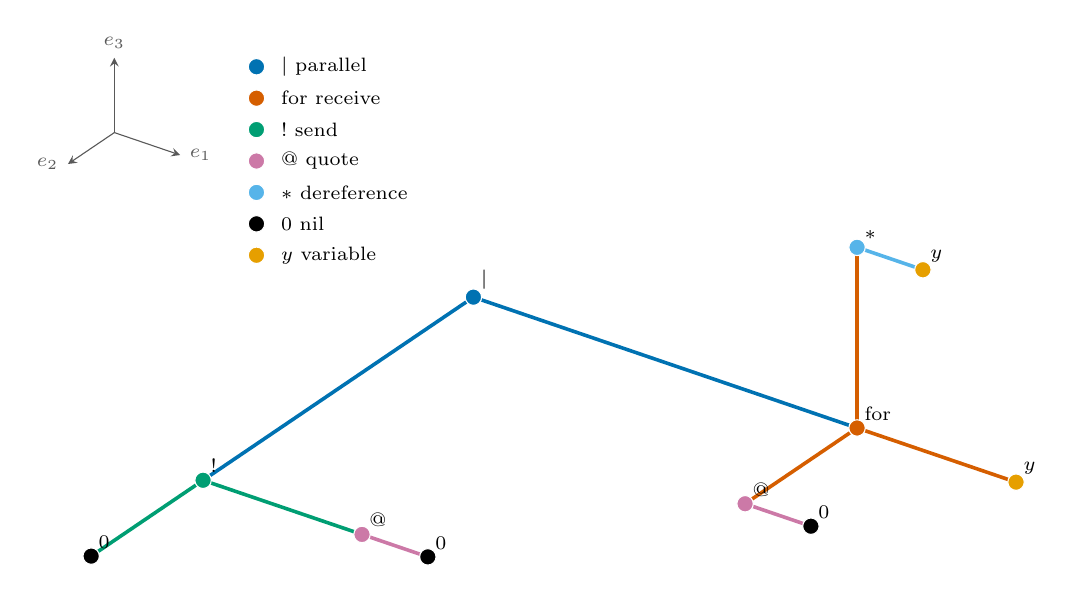
\begin{tikzpicture}[x=0.95cm,y=0.95cm]
  \begin{scope}[shift={(-4.8,2.2)},>=stealth,gray!70!black]
    \draw[->] (0,0)--(0.88,-0.30) node[right]{\scriptsize $e_1$};
    \draw[->] (0,0)--(-0.62,-0.42) node[left]{\scriptsize $e_2$};
    \draw[->] (0,0)--(0,1) node[above]{\scriptsize $e_3$};
  \end{scope}
  \draw[line width=1.3pt,cpar] (0.000,0.000)--(5.129,-1.749);
\draw[line width=1.3pt,crecv] (5.129,-1.749)--(7.254,-2.473);
\draw[line width=1.3pt,crecv] (5.129,-1.749)--(3.632,-2.762);
\draw[line width=1.3pt,cquote] (3.632,-2.762)--(4.512,-3.062);
\draw[line width=1.3pt,crecv] (5.129,-1.749)--(5.129,0.666);
\draw[line width=1.3pt,cdrop] (5.129,0.666)--(6.009,0.366);
\draw[line width=1.3pt,cpar] (0.000,0.000)--(-3.614,-2.448);
\draw[line width=1.3pt,csend] (-3.614,-2.448)--(-1.489,-3.172);
\draw[line width=1.3pt,cquote] (-1.489,-3.172)--(-0.609,-3.472);
\draw[line width=1.3pt,csend] (-3.614,-2.448)--(-5.110,-3.462);
\node[hub,fill=cpar] at (0.000,0.000) {};
\node[lab] at (0.000,0.000) {\scriptsize $\mid$};
\node[hub,fill=crecv] at (5.129,-1.749) {};
\node[lab] at (5.129,-1.749) {\scriptsize for};
\node[hub,fill=cy] at (7.254,-2.473) {};
\node[lab] at (7.254,-2.473) {\scriptsize $y$};
\node[hub,fill=cquote] at (3.632,-2.762) {};
\node[lab] at (3.632,-2.762) {\scriptsize $@$};
\node[hub,fill=c0] at (4.512,-3.062) {};
\node[lab] at (4.512,-3.062) {\scriptsize $0$};
\node[hub,fill=cdrop] at (5.129,0.666) {};
\node[lab] at (5.129,0.666) {\scriptsize $*$};
\node[hub,fill=cy] at (6.009,0.366) {};
\node[lab] at (6.009,0.366) {\scriptsize $y$};
\node[hub,fill=csend] at (-3.614,-2.448) {};
\node[lab] at (-3.614,-2.448) {\scriptsize $!$};
\node[hub,fill=cquote] at (-1.489,-3.172) {};
\node[lab] at (-1.489,-3.172) {\scriptsize $@$};
\node[hub,fill=c0] at (-0.609,-3.472) {};
\node[lab] at (-0.609,-3.472) {\scriptsize $0$};
\node[hub,fill=c0] at (-5.110,-3.462) {};
\node[lab] at (-5.110,-3.462) {\scriptsize $0$};

  \begin{scope}[shift={(-2.9,3.5)}]
    \foreach \c/\n [count=\k] in {cpar/{$\mid$ parallel},crecv/{for receive},csend/{$!$ send},cquote/{$@$ quote},cdrop/{$*$ dereference},c0/{$0$ nil},cy/{$y$ variable}}
      { \node[hub,fill=\c] at (0,-0.42*\k) {}; \node[anchor=west] at (0.2,-0.42*\k) {\scriptsize \n}; }
  \end{scope}
\end{tikzpicture}
\caption{Realisation D of $\mathsf{for}(y\leftarrow @0)\,{*y}\mid @0!(0)$ in
$\R^3$, drawn in axonometric view. Colour names the constructor; the direction of
a spoke names the argument position. The two occurrences of $@0$ are congruent
sub-figures, as are any two occurrences of the same subterm.}\label{fig:rho}
\end{figure}

Three things are visible in the figure and hold in general.
\begin{itemize}
\item \emph{Subterms are congruent sub-figures.} Every occurrence of $@0$ is the
same purple--black segment along $e_1$, so repeated structure is seen as repeated
shape. In particular the channel of the receive and the channel of the send, whose
agreement is the side condition of the COMM rule, are recognisably the same
shape, at $e_2$ of the receive and $e_1$ of the send.
\item \emph{Unary constructors run along $e_1$.} A tower of quotes and
dereferences is a straight line whose colour sequence spells the tower; the hubs
keep its segments apart, which is exactly what failed for stems in
Realisation A.
\item \emph{Binding is not drawn.} The variable $y$ appears as a leaf colour at
its binding occurrence and at its use, and nothing in the geometry links them.
With de Bruijn indices each index would need its own leaf colour instead of its
own axis, so the dimension stays at $3$; an explicit chord from use to binder
is the alternative, and whether it can always be routed without contact is open.
\end{itemize}

\paragraph{Aids to legibility.} Since sizes grow by about $2.4$ per level, line
weight proportional to $\rad$ of the subterm makes depth readable. The bounding
balls are disjoint by construction, so a subterm can be collapsed to its ball
until selected. For signatures with $N>3$ a projection is needed again, but of
$N$ axes rather than $\sum_c(1+\ar(c))$.

\paragraph{What is given up.} ``One dimension per constructor'' now holds in
colour space and not in physical space, and the stem, which in the original
procedure marks the constructor from outside the bounding sphere, becomes a
coloured hub inside it. Realisation D is otherwise the corner construction of
Definition~\ref{def:B} with its blocks superimposed.

\section{Summary}

\begin{enumerate}
\item The stated procedure needs five repairs to be a definition
(Section~\ref{sec:review}); with them it is Realisation A.
\item Realisation A is not an embedding when unary or binary constructors are
present (Proposition~\ref{prop:Afail}), though it distinguished all $485$ test
terms.
\item Moving the hub to the apex over the simplex gives Realisation B, which is an
embedding and decodable (Theorems~\ref{thm:emb}, \ref{thm:faith}) at the cost of
one more axis per constructor and a growth factor of $1+\sqrt2$.
\item Sizes grow exponentially in height in A and B, and contexts do not act
locally. Variant C trades outward growth for inward contraction and makes
contexts similarities.
\item Encoding the constructor as colour and keeping only argument position in
space (Realisation D) is an embedding in $\R^{\max\ar}$
(Theorem~\ref{thm:D}); the rho calculus renders in $\R^3$ without projection
(Figure~\ref{fig:rho}).
\item Open: bound variables, a general proof of faithfulness for A, and whether A
is an embedding when all arities are at least $3$.
\end{enumerate}

\appendix
\section{Reproducing the check}
The script \texttt{check.py} implements Definitions~\ref{def:A} and~\ref{def:B}
with $\gamma=\delta=1$, tests every pair of segments for contact other than at a
shared endpoint, and compares figures as point sets after merging collinear
overlaps. Output: A, dimension $7$, $252/485$ with contact, $0$ coincident pairs;
B, dimension $10$, $0/485$ with contact, $0$ coincident pairs, maximum radius
$80.6=(1+\sqrt2)^5-\sqrt2$; D, dimension $3$, $0/485$ with contact (including
hubs interior to spokes), $0$ coincident coloured hub sets, maximum radius
$23.31=((1+\sqrt2)^4-1)/\sqrt2$. Run as \texttt{python3 check.py fig-rho.tex},
the script also regenerates the coordinates of Figure~\ref{fig:rho}.

\end{document}
